\documentclass[USenglish,oneside,twocolumn]{article}

\usepackage[utf8]{inputenc}%(only for the pdftex engine)
%\RequirePackage[no-math]{fontspec}%(only for the luatex or the xetex engine)
\usepackage[big]{dgruyter_NEW}
% allow URL breaks on dashes
\def\UrlBreaks{\do\/\do-}

% math environment
\usepackage{mathtools}
\usepackage{amsmath}
\usepackage{amssymb}
\usepackage[%
    lambda, advantage, operators, sets, adversary, landau, probability, notions,
    logic, ff, mm, primitives, events, complexity, asymptotics, keys,
]{cryptocode}

% prettier line breaks
\usepackage{microtype}

% figures
\usepackage{graphicx}
\usepackage[position=bottom]{subfig}
\usepackage{tikz}
\usepackage{tikz-qtree}
\usetikzlibrary{shapes.misc,positioning,arrows,snakes,calc}

% colors
\usepackage{color}
\usepackage{colortbl}
\definecolor{rgddTeal}{HTML}{009999}
\definecolor{rgddLime}{HTML}{809933}
\definecolor{rgddPurple}{HTML}{993380}
\definecolor{rgddDred}{HTML}{E04644}
\definecolor{rgddDgreen}{HTML}{008000}
\definecolor{rgddDblue}{HTML}{2809B2}

% custom commands
\newcommand{\TODO}[1]{\textcolor{red}{TODO:} \emph{#1}}

 
\DOI{foobar}

\cclogo{\includegraphics{by-nc-nd.pdf}}
  
\begin{document}
  %\author*[1]{Corresponding Author}
  %\author[2]{Second Author}
  %\author[3]{Third Author}
  %\author[4]{Fourth Author}
  %\author[5]{Fifth Author}
  %\affil[1]{Affil, E-mail: email@email.edu}
  %\affil[2]{Affil, E-mail: email@email.edu}
  %\affil[3]{Affil, E-mail: email@email.edu}
  %\affil[4]{Affil, E-mail: email@email.edu}
  %\affil[5]{Affil, E-mail: email@email.edu}

  \title{\huge%
	Incremental and Privacy-Preserving Certificate Transparency Support Within
	the Tor Network
  }
  \runningtitle{%
	Incremental and Privacy-Preserving Certificate Transparency Support Within
	the Tor Network
  }
  %\subtitle{...}

  \begin{abstract}
      {The security of the web improved greatly throughout the last couple of years.
A large majority of the web is now served encrypted as part of HTTPS, and
web browsers accordingly moved from positive to negative security indicators
that warn the user if a connection is insecure.  A secure connection requires
that the server presents a valid certificate that binds the domain name in
question to a public key.  A certificate used to be valid if signed by a trusted
Certificate Authority (CA), but modern web browsers like Google Chrome and
Apple's Safari additionally started to mandate Certificate Transparency (CT)
logging to overcome the weakest-link security of the CA ecosystem.  Tor and the
Firefox-based Tor Browser have yet to enforce CT.

\hspace{12pt}
In this paper, we present privacy-preserving and incrementally-deployable
designs that add support for CT in Tor. Our designs go beyond the currently
deployed CT enforcements that are based on blind trust:
	if a user that uses Tor Browser is man-in-the-middled over HTTPS,
	we probabilistically detect and disclose cryptographic evidence of CA and/or
	CT log misbehavior.
The first design increment allows Tor to play a vital role in the overall goal
of CT:
	detect mis-issued certificates and hold CAs accountable.
We achieve this by randomly cross-logging a subset of certificates into other CT
logs.  The final increments hold misbehaving CT logs accountable, initially
assuming that some logs are benign and then without any such assumption.
Given that the current CT deployment lacks strong mechanisms to verify if log
operators play by the rules, exposing misbehavior is important for the web in
general and not just Tor.  The full design turns Tor into a system for
maintaining a probabilistically-verified view of the CT log ecosystem available
from Tor's consensus.  Each increment leading up to it preserves privacy due to
and how we use Tor.
}
  \end{abstract}

  \keywords{Certificate Transparency, Tor}
  %\classification[PACS]{}
  %\communicated{...}
  %\dedication{...}

  \journalname{Proceedings on Privacy Enhancing Technologies}
  \DOI{Editor to enter DOI}
  \startpage{1}
  \received{..}
  \revised{..}
  \accepted{..}

  \journalyear{..}
  \journalvolume{..}
  \journalissue{..}
 
  \maketitle
  %\section{Introduction} \label{sec:introduction}
Metrics reported by Google and Mozilla reveal that encryption on the web
skyrocketed the past couple of years: at least 85\% of all web pages load using
Transport Layer Security (TLS) as part of
HTTPS~\cite{google-metrics,mozilla-metrics}. A HTTPS connection is initiated by
a TLS handshake where the client web browser requires that the web server
presents a valid certificate to authenticate the identity of the server (e.g.,
to make sure that the client who wants to visit \url{mozilla.org} really is
connecting to Mozilla, and not, say, Google). A certificate is considered valid
if it is digitally signed by a Certificate Authority (CA) that the browser
trusts. Each CA is trusted to certify (sign) that specific cryptographic
key-material as part of a certificate belongs to a particular domain name.

It used to be costly to obtain a widely trusted certificate in the past, but
Let's Encrypt significantly reduced the barrier towards HTTPS everywhere by
providing free and automated certificate issuance since its launch as a
non-profit CA in 2015~\cite{le}. The current mindset of encryption as default is
evident by other ongoing initiatives too, such as modern web browsers moving
from positive to negative security indicators~\cite{chrome-ui,firefox-ui} and
the rapid deployment of TLS version 1.3~\cite{rapid-tls13}.

The CA trust model suffers from \emph{weakest-link} security: web browsers trust
hundreds of CAs, and it is enough to compromise a single CA to get a certificate
mis-issued in the name of a target domain~\cite{ca-ecosystem,https-sok}.
Motivated by this issue manifested by prominent CA compromises---such as the
issuance of a fraudulent certificate for \url{google.com} by DigiNotar in
2011\footnote{\url{https://web.archive.org/web/20200521135444/https://arstechnica.com/information-technology/2011/08/earlier-this-year-an-iranian/}}---several
major browser vendors have mandated that certificates issued by CAs must be
included into trusted Certificate Transparency (CT) logs for browsers to trust
them~\cite{ct/a,ct,ct/bis}. The idea behind CT is that by making all issued
certificates transparent miss-issued certificates can be detected \emph{after}
issuance and appropriate actions taken to keep the wider web safe (e.g.,
revocation of certificates, suspected compromises investigated, or trust in
misbehaving CAs removed from browsers). Browsers that wish to benefit from CT
augment the validation done by the browser during the TLS handshake to also
require cryptographic proof from the server that the presented certificate has
been included into CT logs trusted by the browser. Notable browsers with
mandatory CT support by default are Google Chrome and Apple's Safari
\cite{chrome-policy,safari-policy}, while Mozilla's Firefox lacks support by
default.

Firefox is the basis for Tor Browser (TB) from the Tor Project~\cite{tor}. TB
enables anyone to browse the web anonymously by relaying traffic between browser
and web server through the Tor network, consisting of thousands of voluntary-run
relays across the globe. There are many techniques an attacker can use to
attempt to deanonymize a TB user, such as end-to-end correlation attacks or
other forms of traffic analysis~\cite{tor, FIXME}. 

One common deanonymization technique---known to be used in practice by, e.g., law
enforcement---is to compromise TB instead of directly circumventing the anonymity
provided by the Tor network~\cite{FIXME}. Modern web browsers like TB (Firefox)
are one of the most complex types of software in wide use today. This complexity
and wide use leads to security vulnerabilities and incentives for exploitation.
For example, the exploit acquisition platform Zerodium offers up to \$100,000
for a zero-day exploit against Firefox that leads to remote code execution and
local privilege
escalation\footnote{\url{https://web.archive.org/web/20200521151311/https://zerodium.com/program.html}}
(i.e., full control of the browser for the attacker).

An attacker that wishes to use such an exploit to compromise and then ultimately
deanonymize a TB user has to deliver the exploit to TB. Since the web is mostly
encrypted today, this primarily has to happen over a HTTPS connection where the
attacker controls the content returned by the web server. While there are a
number of possible ways for an attacker to accomplish this (e.g., by
compromising a web server that the target TB user connects to), one option is to
\emph{impersonate} a web server by acquiring a fraudulent certificate. Due to the
Tor network being run by volunteers, getting into a position for performing such
an attack is relatively straightforward (the attacker can volunteer to run
malicious relays~\cite{spoiled-onions}). The same is true for an attacker that
wishes to \emph{man-in-the-middle} connections made by TB users. In such a case,
a TB exploit may not even be needed to deanonymize the user; e.g., if the user
logs in an account at the service associated with its identity that the attacker
can now observe.

\subsection{Overview of CTor}
We propose a design that enforces CT incrementally in Tor Browser: CTor.  The
three increments are as follows:
\begin{enumerate}
	\item \textbf{Basic CT policy:}
		Tor Browser enforces a basic CT policy that requires promises of public
		CT logging.
	\item \textbf{Resilience towards misbehaving CT logs:}
		Tor Browser is part of a Tor-wide auditing process that adds certificate
		chains in independent CT logs.
	\item \textbf{Detection of misbehaving CT logs:}
		Tor Browser is part of a Tor-wide auditing process that exposes evidence
		of CT logs that misbehaved.
\end{enumerate}

Following Google's suit to minimize CT breakage~\cite{does-ct-break-the-web},
the first step is a leap in the right direction which detects mis-issued TLS
certificates that are presented to Tor Browser users \emph{if all CT logs are
honest}.  This is the same flawed assumption that the CA ecosystem relies on,
and we already observed several instances of CT logs that misbehaved~%
	\cite{izenpe-disqualified,venafi-disqualified,gdca1-omission}.
Most recently, a compromised CT log signing key was reported for the first
time~\cite{digicert-log-compromised}.

To add \emph{resilience} against CT logs that misbehave, we propose a Tor-wide
auditing process.  It is composed of a submission phase, a storage phase, and
an auditing phase:
	Tor Browser submits a presented certificate chain probabilistically to
		a random Tor relay,
	which in turn stores it temporarily before adding it to an independent CT
		log that have yet to promise any public logging.
As such, a certificate chain is likely to make it into the public domain
\emph{if some independent CT logs are benign}.  Section~\ref{sec:todo} motivates
why Tor's threat model makes it difficult to perform CT auditing straight-up
from Tor Browser.  Therefore, Tor relays are part of the process.

The basic design can be extended at the cost of different deployment trade-offs
and trust assumptions, such that it is possible to \emph{detect CT logs that
misbehaved} by omitting a certificate chain from the public.  We propose two
orthogonal extensions.  First, a proposal that shifts trust from CT logs to CT
auditors that are easier to diversify due to different operational
requirements.  Second, a trivial extension of the base design that requires
small, but significant, changes to the CT landscape in the form of an
additional CT log endpoint.

\subsection{Contribution and Structure}

  %\section{Background} \label{sec:background}

\subsection{Certificate Transparency} \label{sec:background:ct}
The idea to transparently log TLS certificates emerged at Google in response to
a lack of proposals that could be deployed without drastic ecosystem changes
and/or significant downsides~\cite{ct/a}.  In reality, CT is about logging
certificate \emph{chains}:
	a domain owner's certificate is signed by an intermediate CA, whose
	certificate is in turned signed by a root CA that acts as a trust
	anchor~\cite{ca-ecosystem}.
The resulting certificate chain is composed of the domain owner's leaf
certificate, the intermediate CA certificate, and the root CA certificate.
Trust anchors are shipped in software, such as web browsers and operating
systems.

\subsubsection{Cryptographic Foundation}
The operator of a CT log maintains a tamper-evident append-only Merkle
tree~\cite{ct,ct/bis}.  At any time, a Signed Tree Head (STH) can be produced
which fixes the log's structure and content.  Important attributes of an STH
include
	the tree head (a cryptographic hash),
	the tree size (a number of entries), and
	the current time.
Given two tree sizes, a log can produce a \emph{consistency proof} that proves
the newer tree head entails everything that the older tree head does.  As such,
anyone can verify that the log is append-only without downloading all entries
and recomputing the tree head.  Membership of an entry can also be proven
by producing an \emph{inclusion proof} for an STH\@.  These proof techniques are
formally verified~\cite{secure-logging-and-ct}.

Upon a valid request, a log must add an entry and produce a new STH that covers
it within a time known as the Maximum Merge Delay (MMD), e.g., 24~hours.  This
policy aspect can be verified because in response, a Signed Certificate
Timestamp (SCT) is returned.  An SCT is a signed promise that an entry will
appear in the log within an MMD.  A log that violates its MMD is said to perform
an \emph{omission attack}.  It can be detected by challenging the log to prove
inclusion.  A log that forks, presenting one append-only version
to some entities and another to others, is said to perform a \emph{split-view
attack}.  Split-views can be detected by STH
gossip~\cite{chuat,dahlberg,nordberg,syta}.

\subsubsection{Standardization}
The standardized CT protocol defines public HTTP(S) endpoints that allow anyone
to check the log's accepted trust anchors and added certificates, as well as
obtaining the most recent STH and fetching proofs~\cite{ct,ct/bis}.  For
example, the \texttt{add-chain} endpoint returns an SCT if the added certificate
chain ends in a trust anchor returned by the \texttt{get-roots} endpoint.  We
use the \texttt{add-chain} endpoint in Section~\ref{sec:base}, and the
\texttt{get-proof-by-hash} as well as the \texttt{get-sth} endpoints in
Section~\ref{sec:auditor}.  The \texttt{get-proof-by-hash} endpoint takes as
input a leaf certificate hash and an STH's tree size, which indicates the tree
head that the log should base its inclusion proof on.  The proof is valid if it
can be used in combination with the certificate to reconstruct the tree head of
some STH.

\subsubsection{Verification}
The CT landscape provides a limited value unless it is verified that the logs
play by the rules.  The rules are largely influenced by major browser vendors
that define CT policies.  For example, how is CT enforced by their user agents,
and what is required to become a recognized CT log in terms of uptime
requirements and accepted trusted anchors.  Google's Chrome and Apple's Safari
require that a certificate chain must be accompanied by two independent
SCTs~\cite{chrome-policy,safari-policy}.  Independence refers to the associated
log operators.  While there are several ways that
a log can misbehave with regards to these policy aspects, the most fundamental
forms of cheating are omission and split-view attacks:
	it would undermine detection of mis-issued TLS certificates.
A party that follows-up on inclusion and consistency proofs is said to
\emph{audit} the logs.  Wide-spread client-side auditing is a premise for CT
logs to be untrusted, but none of the web browsers that enforce CT engage in
such activities yet.  For example, it is difficult due privacy
concerns~\cite{ct-with-privacy}.  CT also assumes that domain owners
\emph{monitor} the logs for mis-issuance by inspecting the added
certificates~\cite{lwm,ct-monitors}.

\subsection{Tor} \label{sec:background:tor}

Most of the activity of Tor's millions of daily users starts with Tor Browser
(TB) and connects to some ordinary website via a circuit comprised of three
randomly-selected Tor relays. In this way no identifying information from
Internet protocols (such as IP address) are automatically provided to the
destination, and no single entity can observe both the source and destination of
a connection. TB is also configured and performs some filtering to resist
browser fingerprinting, and first party isolation to resist sharing state or
linking of identifiers across origins. More generally it avoids storing
identifying configuration and behavioral information to disk.

Tor relays in a circuit are selected at random, but not uniformly. A typical
circuit is comprised of a \emph{guard}, a \emph{middle}, and an \emph{exit}. A
guard is selected by a client and used for several months as the entrance to all
Tor circuits. If the guard is not controlled by an adversary, that adversary
will not find itself selected to be on a Tor circuit adjacent to (thus
identifying) the client. And because some relay operators do not wish to act as
the apparent Internet source for connections to arbitrary websites, relay
operators can configure the ports (if any) on which they will permit connections
besides to other Tor relays. Finally, to facilitate load balancing, relays are
assigned a weight based on their apparent capacity to carry traffic. In keeping
with avoiding storing of linkable state, even circuits that share an origin will
only permit new connections over that circuit for ten minutes. After that, if
all connections are closed, all state associated with the circuit is cleared.
Similarly, at each relay state associated with a given circuit is cleared
shortly after a circuit is closed.

Tor clients use this information when choosing relays with which to build a
circuit. They receive the information via an hourly updated \emph{consensus}.
The consensus assigns weight as well as flags such as \texttt{guard} or
\texttt{exit} along with auxiliary flags such as \texttt{stable}, which, e.g.,
is necessary to obtain the \texttt{guard} flag since guards must have good
availability. Self-reported information by relays in their \emph{extra-info
document}, such as statistics on their read and written bytes, are also part of
the consensus and uploaded to \emph{directory authorities}. Directory
authorities determine the consensus by voting on various components making up
the shared view of the state of the Tor network. Making sure that all clients
have a consistent view of the network prevents epistemic attacks wherein clients
can be separated based on the routes that are consistent with their
understanding~\cite{danezis:pets2008}. This is only a very rough sketch of Tor's
design and operation.  More details can be found by following links at Tor's
documentation site~\cite{tor-documentation}.

Tor does not aim to prevent end-to-end correlation attacks. An adversary
controlling the guard and exit, or controlling the destination and observing the
client ISP, etc. is assumed able to confirm who is connected to whom on that
particular circuit. The Tor adversary model assumes an adversary able to control
and/or observe a small to moderate fraction of Tor relays measured by both
number of relays and by consensus weight, assumes a large number of Tor clients
able to, for example, flood individual relays to detect traffic signatures of
honest traffic on a given circuit~\cite{long-paths}. Also, the adversary can
knock any small number of relays offline via either attacks from clients or
direct Internet DDoS\@. 

  %\section{Threat Model} \label{sec:adversary}
%
% Attacker capabilities
%
We consider an attacker that controls
	a CA,
	enough CT logs to pass Tor Browser's SCT-centric CT policy, 
	some Tor clients, and
	a moderate fraction of Tor relays.
For example, it is possible to
	issues certificates and SCTs,
	dishonor promises of public logging,
	present split-views at will,
	intercept and delay traffic from controlled exit relays as well as CT logs,
		and
	be partially present in the network.
Note that this includes a weaker attacker that does not \emph{control} CAs and
CT logs, but, who gained access to their signing
keys~\cite{turktrust,gdca1-omission}.
A subset of CTor entities can be subject to DoS, but not everyone at once and
all the time.  In other words, we consider the threat model of Tor and Tor
Browser as a starting point~\cite{tor,tor-browser}.  It assumed that the
attacker knows all Tor relay configurations, e.g., available memory and setup of
torlog.

%
% Attacker goal and mindset
%
Given that we are in the business of enforcing CT, the attacker needs to hide
mis-issued TLS certificates and SCTs from entities that audit the CT landscape.
As described in Section~\ref{sec:background:ct}, this can either be achieved by
omission or slit-view attacks.  Our intended attacker is clearly powerful and may
successfully issue a certificate chain and associated SCTs without detection
some of the time, but, a CA caught in mis-issuance or a CT log that violated an
MMD promise will no longer be regarded as trusted.  Therefore, we assume a
\emph{risk-averse} attacker that above a relatively low probability of detection
would be deterred from engaging in such activities.

%
% - Our goal: detect TB HTTPS MitM
% - Why: it is a reasonable prerequisite to conduct attacks against TB users
%
We want to minimize the existence of successful man-in-the-middle attacks
against Tor Browser where it cannot be established if
and how they were carried out.  The property of \emph{detection} is inherited
from CT's threat model, which aims to remedy certificate mis-issuance
\emph{after the fact}; not prevent it~\cite{ct/a}.  We
focus on HTTPS traffic that Tor Browser generated because Tor is used to browse
the normal (encrypted) web~\cite{mani}.  Note that it is generally
\emph{difficult} to target a specific Tor Browser user due to Tor's anonymity,
circuit isolation, and HTTPS everywhere.  However, targeting some or all 
users that visit a website is an eminent threat:
	simply intercept traffic from an exit relay or
	upstream of the website.
Once network traffic can be intercepted, it is trivial to serve an exploit to a
subset of Tor Browser users and much easier to target an identifiable user.
Such zero-day exploits are considered in our threat model because \emph{user
exploitation} is the primary reason to attack Tor Browser.

%
% Defer introducing threats that follow from design details
%
We identify additional threats that follow from our adversary model and
design throughout the paper.  For example, the attacker may attempt to
\emph{flood} a Tor relay's submission endpoint to the extent that some
submission must be deleted, i.e., by posing as a Tor Browser user.  If enough
submissions are deleted, the attacker builds up confidence that stored evidence
of CA and CT log misbehavior will not be audited in phase~3
(Section~\ref{sec:todo}).

%%% Local Variables: 
%%% mode: latex 
%%% TeX-master: "../main"
%%% End:          

  %\section{Design} \label{sec:base}
First we introduce a minimal design that makes use of the existing CT landscape
to force certificates into the public domain.  The idea can be viewed as
three phases:
	an SFO is presented to Tor Browser which submits it to a random CTR,
	a submitted SFO is mixed and stored temporarily, and then
	a mixed SFO's certificate chain is submitted for logging in an independent
		CT log.
These phases are depicted further in Figure~\ref{fig:design-ca}, and governed by
parameters that are agreed-upon in the Tor consensus.

Note that our starting point is to chase misbehaving CAs rather than
misbehaving CT logs.  We assume that some, but not all CT logs, are benign
(see Section~\ref{sec:adversary}).

\begin{figure*}
	\centering
	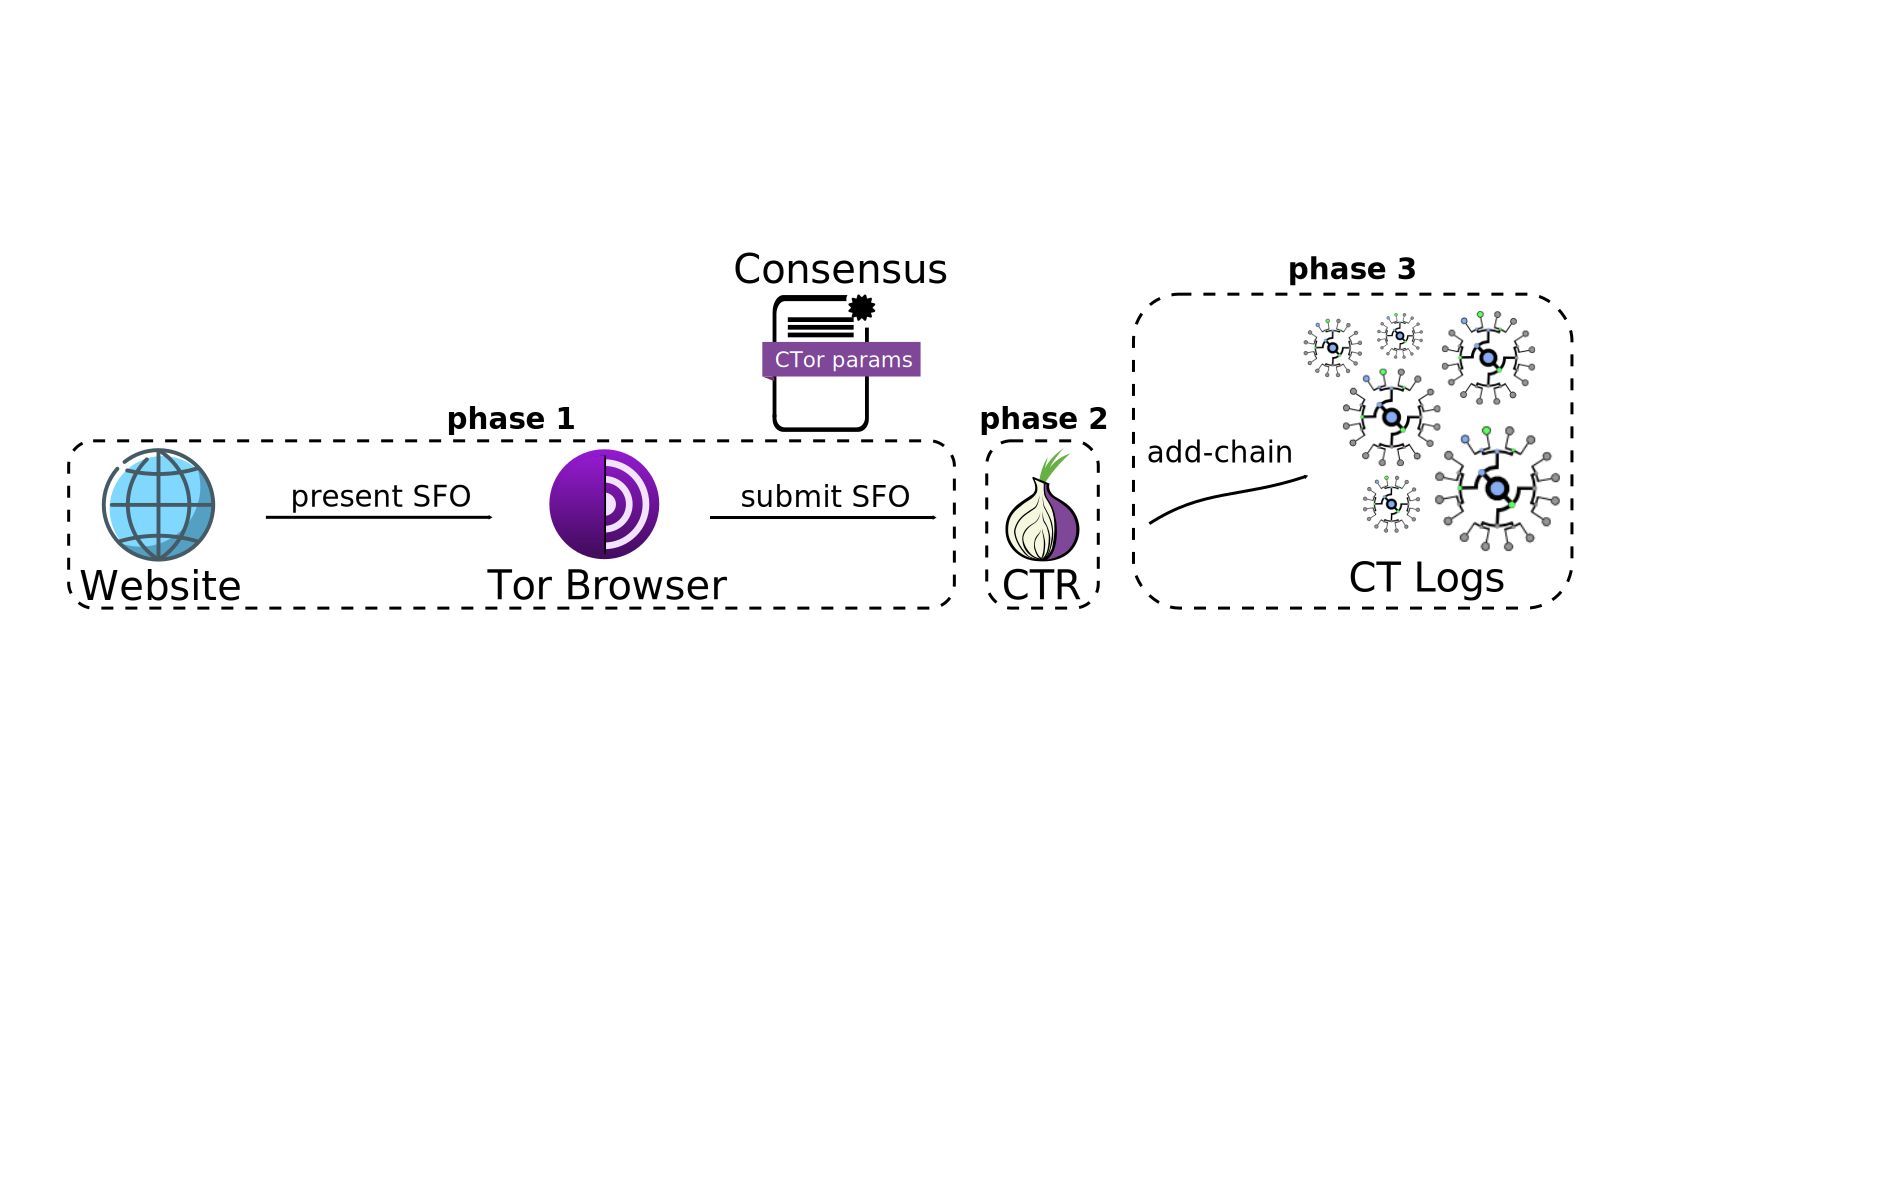
\includegraphics[width=0.85\textwidth]{img/design-ca}
	\caption{An overview of our design: TODO. }
	\label{fig:design-ca}
\end{figure*}

\subsection{Tor Consensus} \label{sec:base:consensus}
Our proposal extends Tor's consensus document
so that it entails information regarding
	CTRs,
	recognized CT logs, and
	other necessary parameters that can be tuned.

\subsubsection{CTR Flag} \label{sec:base:consensus:ctr-flag}
The existing \texttt{known-flags} item determines the different flags that a 
given consensus document might contain.  We add another flag named \texttt{CTR},
which indicates that a relay should support CT-auditing as described in
Sections~\ref{sec:base:phase2}--\ref{sec:base:phase3}.  A relay qualifies as a
CTR if it is flagged as \texttt{stable} and \texttt{middle}, which means that we
suggest using resources that are more abundant when compared to, for example,
exit bandwidth.  A Tor relay is assigned the \texttt{CTR} flag if a majority of
directory authorities voted~for~it.

\subsubsection{Recognized CT Log} \label{sec:base:consensus:log}
CTRs only interact with CT logs that are recognized by the Tor consensus.  A log
is recognized if a majority of directory authorities voted for its inclusion by
proposing a \texttt{ct-log-info} entry that contains a log ID, a public key, and
a base URL~\cite{ct,ct/bis}. 
Following from our basic CTR design, there need not be any overlap between the
logs that the Tor consensus recognizes when compared to Tor Browser's CT policy.
There could be overlap, however.  The ideal scenario is that there are many
independent logs that accept certificate chains for most trust anchors.

For now, we do not provide any details as to how the Tor consensus captures
whether two logs are independent or which trust anchors they accept.
Section~\ref{sec:discussion:logs} discusses this and other related
considerations further.

\subsubsection{Other Parameters} \label{sec:base:consensus:params}
Directory authorities influence the way in which Tor Browser and CTRs behave by
voting on other necessary parameters.  For example, the likelihood that
an SFO is submitted for further auditing is a security parameter that is
determined by the value of \texttt{ct-submit-pr}.  The value of an item is
computed as the median of all votes.
\begin{description}
	\item[ct-submit-pr:] A floating-point in $[0,1]$ that determines Tor
		Browser's submission probability, i.e., whether an SFO should be sent to
		a random CTR for further auditing.  Zero disables auditing,
		while $0.10$ implies every 10$^{\mathsf{th}}$ SFO is audited
		on average.
	\item[ct-sfo-max-bytes:] A natural number that determines how many
		wire-bytes a normal SFO should not exceed.  As outlined in
		Section~\ref{sec:base:phase1}, excessively large SFOs are subject
		to stricter verification criteria.
	\item[ct-query-timeout:] A natural number that determines how many ms a CTR
		waits before concluding that a CT log is unresponsive.  As outlined in
		Section~\ref{sec:base:phase3}, a query timeout triggers a
		resubmission later on.
	\item[ct-backoff:] A natural number that determines how many ms a CTR
		may wait between two auditing instances.  As outlined in
		Section~\ref{sec:base:phase3}, CTRs audit pending SFOs
		in batches at random time intervals.
	\item[ct-delay-dist] docdoc
\end{description}


\subsection{Phase~1---Tor Browser} \label{sec:base:phase1}
The first phase evolves around Tor Browser and how an incoming SFO is validated
and probabilistically audited further by a random CTR.  Given an SFO $s$ and
a tab $t$:
\begin{enumerate}
	\item Accept $s$ and stop if it was already validated in $t$.
	\item Raise a certificate error and stop if the certificate chain of $s$
		is not rooted in Tor Browser's trust store.
	\item Raise a certificate transparency error and stop if the SCTs of $s$
		fail Tor Browser's SCT-centric CT policy.
	\item Mark $s$ as validated in $t$ and continue in the background if
		$\mathsf{len}(s) \le \texttt{ct-max-sfo-bytes}$, else continue in
		blocking-mode before marking $s$ as validated in~$t$.
	\item Flip a biased coin based on \texttt{ct-submit-pr} and stop if the
		outcome indicates no further auditing.
	\item Submit $s$ to a sampled CTR's SFO-endpoint on a pre-built CT-circuit
		that starts from the client's guard and ends at the CTR: three hops in
		total.  The circuit used for submission is closed immediately after
		use without waiting for any acknowledgment.
\end{enumerate}

We avoid unnecessary overhead by only validating SFOs once per tab.  An SFO is
considered validated if the end-entity certificate is rooted in a trust anchor
\emph{and} it has enough SCTs as dictated by an SCT-centric CT policy which is
similar to the other major browser vendors~\cite{chrome-policy,safari-policy}.
Section~\ref{sec:analysis} motivates why excessively large SFOs are vetted more
strictly in blocking-mode, which is in contrast to the normal behavior where an
SFO is considered for further auditing in the background.  Moreover, note that
the circuit used to submit an SFO is taken from a pool of pre-built CT-circuits
that are closed immediately after use, reducing the time that they are around in
memory.

%
% - close circuit asap to make it harder for an attacker to figure out which
% CTR received a submission (should it have access to a zero-day takeover).
% - clearly a submission circuit cannot be reused across tabs, but not doing
% so within tabs may (i) reduce the chance that the receiving CTR knows exactly
% which website was visited, and (ii) make sense because with small submission
% pr (<=1/10) it should be common to submit at most once per tab anyway.
%

\subsection{Phase 2---CTR Storage} \label{sec:base:phase2}
We suggest that CTRs accept SFO submissions on an HTTP endpoint.\footnote{%
	Tor's HTTP DirServer codebase can be reused as extension point to interact
	with the tor daemon, i.e., add another listener.
} For example, Nordberg~\emph{et~al.} defined an SCT feedback interface that can
be reused if an array-length of one is enforced by the CTR~\cite{nordberg}.
With regards to some circuit, process an incoming SFO $s$ as follows:
\begin{enumerate}
	\item\label{enm:ctr-api:close} Close the incoming circuit.
	\item\label{enm:ctr-api:unrecognized} Stop if no CT log in the Tor consensus
		accepts the underlying certificate chain of $s$.
	\item\label{enm:ctr-api:cached}
		Stop if $s$ is cached or pending to be audited already.
	\item\label{enm:ctr-api:audit-after} Compute an \texttt{audit\_after}
		timestamp $\textrm{t} \gets \mathsf{now()} +
			\mathsf{random\_delay}(\texttt{ct-delay-dist})$.
		The former returns the current time and the latter a random delay.
	\item\label{enm:ctr-api:store}
		Add $s$ and its \texttt{audit\_after} timestamp to a buffer of
		pending SFOs that is managed by tor's OOM.
\end{enumerate}

Recall that Tor Browser does not wait for any acknowledgment, and that a
CT-circuit must not be used more than once.  As such, the first step is to
close the incoming circuit once an SFO is received.  The received SFO is
simply discarded if it
	cannot be audited as proposed in Section~\ref{sec:base:phase3},
	is already audited as noted by a cache, or
	is pending to be audited in a buffer of pending SFOs.
For example, the cache could be a collection of SFO hashes and the buffer
something similar to how OOM manages DNS.  A new SFO is stored in the CTR's
buffer alongside an \texttt{audit\_after} timestamp, which specifies the
earliest point in time that the SFO will be audited.  This behavior, where a
random delay is added to each SFO, transforms the CTR into a timed mix such that
less real-time information is leaked to the CT logs in
Section~\ref{sec:base:phase3}.

If memory becomes a scarce relay resource, e.g., due to flooding, OOM
should delete SFOs at random~\cite{nordberg}.  The threat of flooding is
discussed further in Section~\ref{sec:analysis}.

\subsection{Phase 3---Auditing} \label{sec:base:phase3}
CTR auditing is initiated at random time intervals to spread out the load
imposed by the Tor network on CT logs.  Each auditing instance is composed of
circuit setup, a core loop of SFO enumeration, and circuit tear-down.

\begin{enumerate}
	\item\label{enm:ctr:audit:backoff} Sample a uniform delay from
			$[0, \texttt{ct-backoff}]$,
		then schedule a timer and wait until that time elapsed.
	\item\label{enm:ctr:audit:log-circuit} Establish a new circuit and use it
		for all subsequent log connections.  Connect to the logs when needed.
	\item\label{enm:ctr:audit:loop} Enumerate the buffer of pending SFOs:
		\begin{enumerate}
			\item\label{enm:ctr:audit:too-soon} Continue the loop if
				$\textrm{SFO}.\mathsf{audit\_after} > \mathsf{now}()$.
			\item\label{enm:ctr:audit:sample}
				Sample a log uniformly at random that accepts the underlying
				certificate chain $c \in s$.  Do not consider any log that the
				SCTs of $s$ refer if the Tor consensus lists any independent
				log.
			\item\label{enm:ctr:audit:log} Use \texttt{ct-query-timeout} to set
				a timer and submit $c$ for public logging to the log's
				\texttt{add-chain}~\cite{ct} or
				\texttt{submit-entry}~\cite{ct/bis} endpoint.
				\begin{itemize}
					\item\label{enm:ctr:audit:log:success} On valid
						SCT: cache the SFO, then discard it from the buffer of
						pending SFOs.
					\item\label{enm:ctr:audit:log:fail} On any other outcome:
						break the loop.
				\end{itemize}
		\end{enumerate}
	\item\label{enm:ctr:audit:teardown} Close all opened circuits and go back to
		step~\ref{enm:ctr:audit:backoff}.
\end{enumerate}

As shown above we take an unusual approach towards auditing SFOs.  Rather than
following up on an SCT's inclusion status, we submit the underlying
certificate chain to an independent CT log.  As such, the end-entity certificate
will make it into the public domain if the sampled log is not controlled by the
attacker.  If there is no independent log listed in the Tor consensus, it is
still valuable to resubmit to a dependent log:
	it might be the case that the attacker has access to a log's signing key,
	but not the log's actual infrastructure.
In other words, a mis-issued certificate would make it into the public domain in
such a scenario if we resubmit it rather than discarding it due to lack of
an independent log.

After a certificate chain is submitted for logging, the returned SCT must be
valid, e.g., correct structure and signed by the log in question.  On any other
outcome, such as a timeout, the SFO remains in the buffer of pending SFOs while
the CTR goes into back-off mode.

% TODO: should we fixate so that resubmission to the same sampled log?
% TODO: is it really motivated to "break" now rather than "continue"?

  %\section{Security Analysis} \label{sec:analysis}
TODO: risk, security of base design

  %\section{Auditor Extension} \label{sec:auditor}

%
% Tor consensus
% - At minimum, same logs as Tor Browser's CT policy
% - Need STH+MMD in ct-log-info, not log's public key
% - Need auditors' public keys pinned
% - Need watchdog timeout
% - Need auditor timeout
%

%
% Phase 1---Tor Browser
% - No changes
%

%
% Phase 2---Storage
% - Small differences
%   --> discard unrecognized SCTs based on ct-log-info entries (change step 2).
%   Note entirely sure if this makes that much of a difference tho with regards
%   to flushing, as the attacker can stuff their submissions large anyway...
%   But it makes the next steps easy, as we only have recognized SCTs around.
%   --> sample one SCT, note down the outcome (add step 3.5)
%   --> compute audit after timestamp based on MMD (change step 4)

%
% Phase 3---Auditing
% - Major differences
%   --> establish connection to a random watchdog (add step 1.75)
%   --> step 3 needs a complete rewrite from (b) and forward
%
% Step 3
% b) continue if SFO.audit_after > STH.timestamp
% c) Submit SFO to watchdog
% d) Use ct-query-timeout and STH.treesize to set a timer and challenge the log
% to prove inclusion.
% - On valid proof: send ACK to watchdog, cache SFO, discard SFO from buffer
% - On any other outcome: discard SFO and break the loop
%
% Behavior of watchdog:
% - Listen for submissions on a dedicated endpoint
% - If a submitted SFO is not ACKed within the watchdog timeout
%   --> submit it to an announced auditor.
%   --> resubmit later on if auditor(s) unavailable; not entirely sure which
%   details we should go with here for the resubmission(s)
%

%
% Extra-info document
% - Need flushing statistics
%

%
% MISC notes
% - Network-wide flush, detectable but hard to attribute
% - Requires new reliable auditor software
% - Bit more bandwidth due to watchdog.  The overhead, when compared to log a
% log extension, is sending an SCT hash and receiving a proof (2-3KiB).
%


\begin{figure*}
    \centering
    \includegraphics[width=0.85\textwidth]{img/design-auditor}
    \caption{todo}
    \label{fig:design-auditor}
\end{figure*}

  %\section{Log Extension} \label{sec:log}
If we allow small---yet significant---changes to the CT landscape, it is
possible to avoid inclusion verification and the involved complexities as
described in Section~\ref{sec:auditor}.  The idea is based on returning back to
the premise of some CT logs being honest, and the goal is not only
\emph{resilience towards} but also \emph{detection of} CT logs that misbehaved.
The extended design is nearly identical to the base described in
Section~\ref{sec:base}.
	Tor Browser submits presented SFOs probabilistically to randomly selected
		CTRs in phase 1,
	which store the submitted SFOs in phase 2 before any auditing takes place in
		phase 3.
Here, \emph{auditing} refers to adding a \emph{full SFO} to an independent CT
log; not just the underlying certificate chain.  This is the main difference in
our extension.  By also adding the SCTs, the associated CT logs can be held
accountable.

The prerequisite for such an extension to work is that CT logs support an
additional API endpoint:
	\texttt{add-sfo}.
First we describe how this endpoint could be operated so that \emph{the only
change} is that certificate chains and SCTs are added.  Next, we explain how
some complexity could be moved into Tor but at the cost of bringing back the
threat of flooding (see Section~\ref{sec:auditor:analysis:phase2}).

\textbf{Approach~1.}
Recall from Section~\ref{sec:auditor:design:phase2} that there must not be any
early signals that allow misbehaving CT logs to reactively merge certificate
chains before any MMD promise is violated.  To ensure that this is the case, the
\texttt{add-sfo} endpoint could entail a promise that the added SFO will not be
merged until all MMDs elapsed and the logs (should have) produced STHs that
captured the omission.  For example, the SCT that is returned by the
\texttt{add-sfo} endpoint could have a timestamp that is future-dated by at
least two MMDs, and then it is not considered for merging until that timestamp
is in the present.  The appeal of \emph{delayed merges} is that SFOs need not
be stored any longer than what is necessary for privacy, completely avoiding
the threat of network-wide flushes within our threat model.  Viz., the analysis
in Section~\ref{sec:base} applies without modifications, expect that misbehaving
CAs \emph{and} CT logs are exposed.

\textbf{Approach~2.}  The other option is to make minimal changes to the CT
landscape by operating the \texttt{add-sfo} endpoint without any other
expectation than that it must allow SCTs in addition to a certificate chain.
To avoid early signals, CTRs should employ the same delay strategy as suggested
for CT logs above:
	wait at least two MMDs before adding a (newly issued) SFO.
This is essentially the same as an attacker that maximized the storage phase
by waiting until the last second to produce an STH as discussed in
Section~\ref{sec:auditor:analysis:phase2}, expect that such behavior is assumed
rather than confirmed.  Clearly this brings flooding back to the table, and CTRs
need the extra-info metrics from Section~\ref{sec:auditor:extra-info} to
allow detection.

  %\section{Discussion} \label{sec:discussion}

\subsection{Privacy}
At least mention privacy leaks to auditor. For example, related to CT logs uptime.
  \section{Related Work} \label{sec:related}

%Paul: mixing?

  %\section{Conclusion} \label{sec:conclusion}
CTor consists of a base design and two possible extensions with the goal of
adding incrementally deployable and privacy-preserving support for Certificate
Transparency to Tor. The use of relays in the Tor network distributes caching of
observed SFOs and delays interactions with CT logs, central to both overall
security and preserving privacy of Tor users. Our analysis also shows that these
relays are the weakest link: the most promising chance of avoiding exposure of
compromising SFOs appears to be to attempt to perform network-wide DoS on
relays, or attack CT logs directly. 

Mitigation of network-wide attacks take us outside of Tor's---and therefore also
our---threat model. That said, we cannot ignore such attacks given the strong
attacker we consider (to some degree in control of both a trusted CA and CT
logs). Several parameters of our design enables Tor to \emph{adapt} to observed
interference with CTor, such as a network-wide DoS of relays, reported targeted
attacks of CT logs, or relays reporting suspected flooding through the
\texttt{ct-delete-bytes}  extra-info. When it comes to TB, the submission
probability (\texttt{ct-submit-pr}) and SFO size threshold
(\texttt{ct-max-sfo-bytes}) could be set such as to force all SFOs to be sent to
a CTR before accepting any new HTTPS application-layer data. During the storage
phase, the consensus specifies each CT log's MMD and the delay distribution
(\texttt{ct-delay-dist}), which can be set to either minimize or maximize the
delay between TB user and CT log interaction. Similarly, trusted auditors
(auditor extension) and log operator relationships (base design and log
extension) are also defined in the consensus and can be tweaked.

Deploying CTor, in particular with the log extension that requires trusted
auditors, would be a significant operational burden. Overall Tor network health
would have to include considerations of tweaking CTor parameters to adapt to
strong attackers. However, the potential gains are significant. Tor users would
benefit from the significant security improvement provided by CT logs. Perhaps
more significantly, Tor would be a system for maintaining a
probabilistically-audited cryptographically-verifiable view of the entire CT log
ecosystem available from Tor’s consensus. This would benefit the wider web and
Internet, since the view from Tor's consensus could serve as a base of trust,
relaxing the necessary trust that currently has to be placed on CT log
operators. As a starting point, our base design turns Tor Browser into a helpful
participant in addressing the weakest-link issue of the CA ecosystem, in line
with the goals of CT.


  \bibliographystyle{abbrv}
  \bibliography{src/ref}

  %\appendix
  %\section{Extra}
\end{document}
